
%-------------------------------------------------------------------------------
%							SECOND SECTION
%-------------------------------------------------------------------------------

\section{Presentation of \phifem}

\subsection{The classic FEM framework}
\begin{frame}
    \frametitle{What is FEM?}

    \begin{figure}
        \centering
        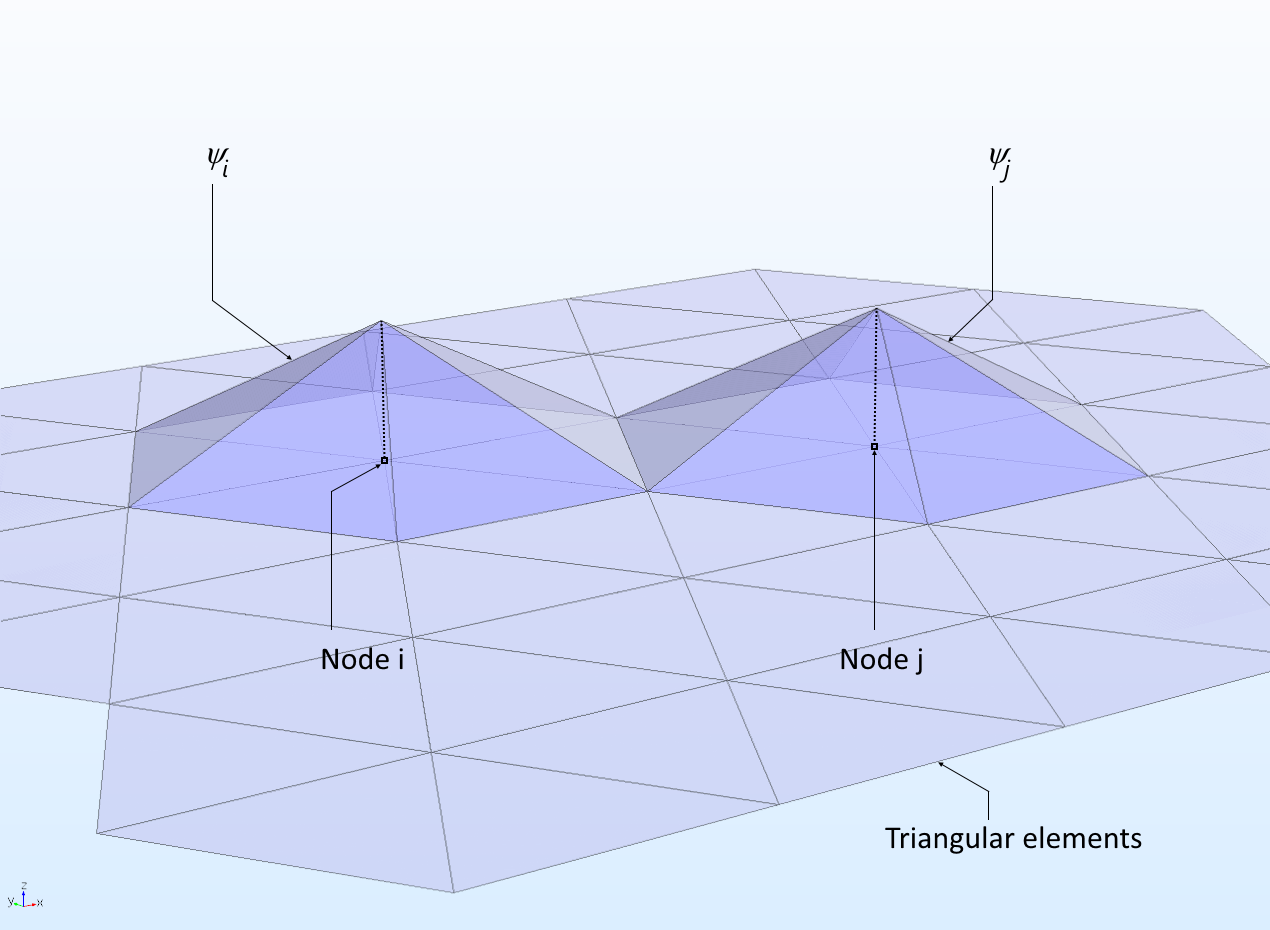
\includegraphics[width=0.8\textwidth]{FEM.png}
        \caption{Finite Elements Method (FEM) principle (\cite{cyclopedia}).}
    \end{figure}

\end{frame}



\subsection{Immersed boundary methods}


\begin{frame}

\frametitle{What are immersed boundary methods?}


\begin{wrapfigure}{r}{0.55\textwidth}
    \includegraphics<4>[width=0.9\linewidth]{XFEM.png} 
    \includegraphics<5>[width=0.8\linewidth]{CutFEM} 
    \includegraphics<6>[width=0.9\linewidth]{SBM} 
    \includegraphics<7>[width=0.9\linewidth]{PhiFEM} 
    \centering
    \only<4>{\caption{XFEM}}
    \only<5>{\caption{CutFEM}}
    \only<6>{\caption{SBM}}
    \only<7>{\caption{\phifem}}
    % \caption{\only<4>{XFEM}\only<5>{CutFEM}\only<6>{SBM}}
    \label{fig:immersed}
\end{wrapfigure}


Immersed boundary methods can handle:
\begin{itemize}
    \item complex geometries \pause
    \item non-body conforming grids \pause
    \item moving/evolving boundaries
\end{itemize}

\pause
Common examples are:
\begin{itemize}
    \item \textbf{XFEM} \parencite{de2018delamination}  \pause
    \item \textbf{CutFEM} \parencite{burman2015cutfem}\pause
    \item \textbf{SBM} \parencite{atallah2020analysis} \pause
    \item \textbf{\phifem}\parencite{Reference3}
\end{itemize}

\note{Les 3 premieres methodes demandes des integrations sur la forntiere. PhiFEM ne demande pas de telle integrations; la quadrature se passe sur la frontiere fictive.}

\end{frame}


\begin{frame}
    \frametitle{What is \phifem?}
The main ideas are (for Dirichlet boundary conditions): 
\begin{enumerate}
    \item \textbf{Define the domain using a level-set function $\phi$.}
    \item \textbf{Then make that function carry the solution: $u = \phi w + g$.}
\end{enumerate}
 
\begin{figure}
    \centering
    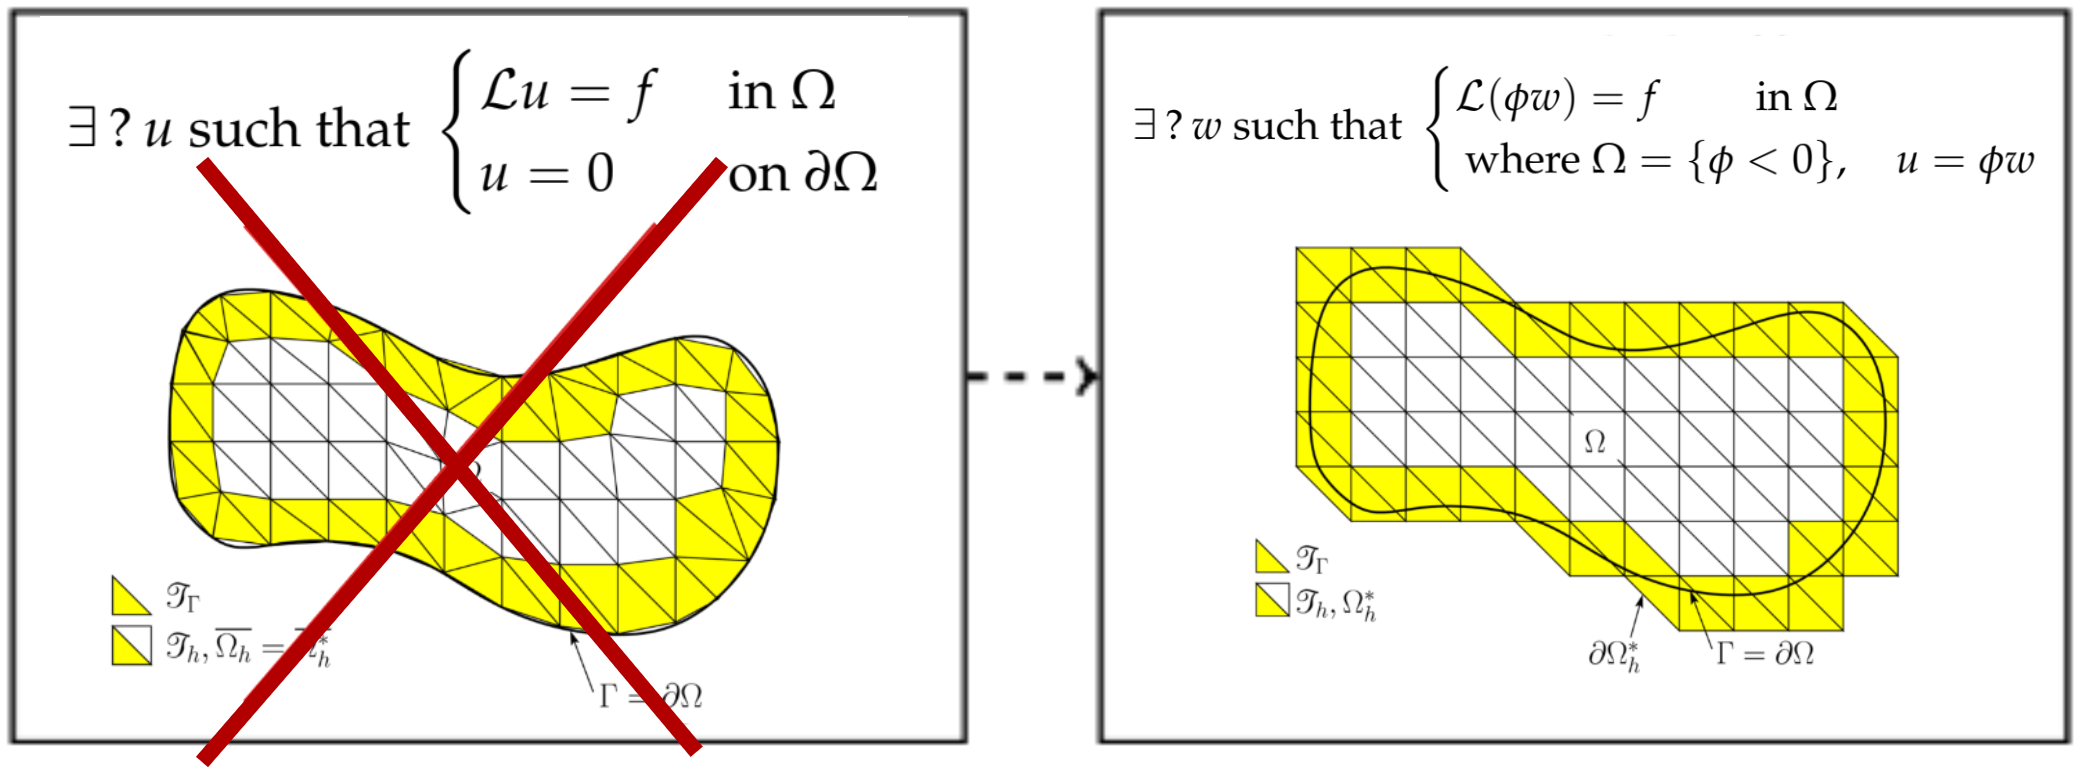
\includegraphics[width=0.95\textwidth]{ClassicToPhiFEM.png}
    \caption{From Classic FEM (on the left) to \phifem (on the right)}
\end{figure}
\end{frame}

